\begin{question}
\noindent Mission control is tracking a satellite as it moves through two stages of a course correction, plotted on a coordinate grid where each unit represents 100 km.

\noindent The satellite starts at point $S(2,1)$.

\medskip
\noindent \textbf{Stage 1:} The satellite fires its thrusters and translates by the vector $\begin{pmatrix} 3 \\ -4 \end{pmatrix}$ to reach point $S'$.

\noindent \textbf{Stage 2:} The satellite then performs a rotation of $90^\circ$ clockwise about the origin $O$ to reach its final tracking position $S''$.

\begin{center}
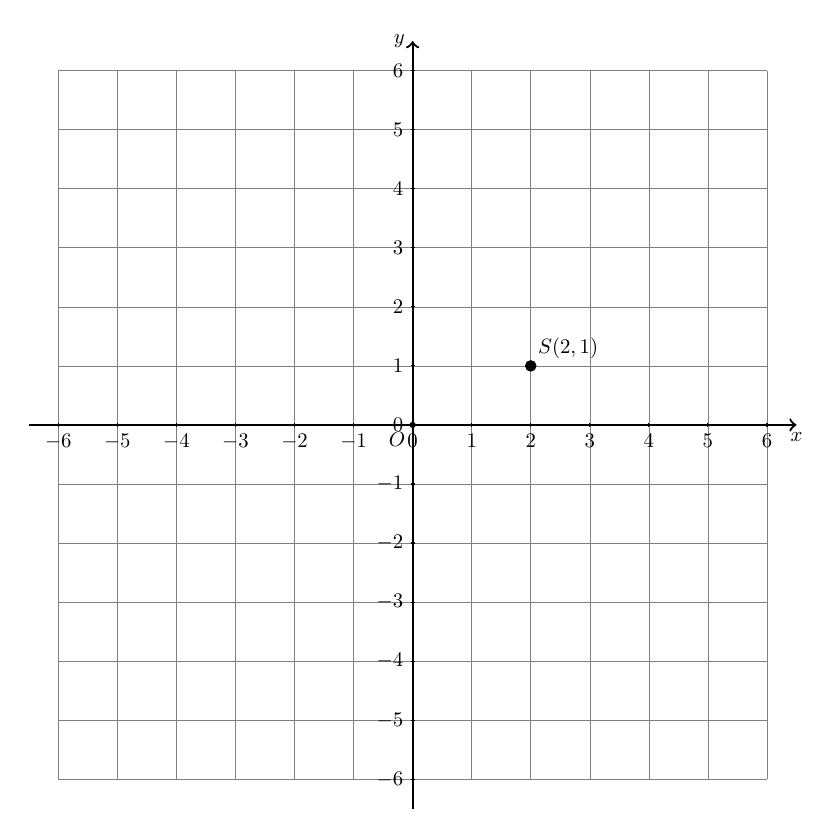
\begin{tikzpicture}[scale=0.75, transform shape]
    \def\axisLimit{6}
    \definecolor{borderColour}{HTML}{000000}

    % Draw grid
    \draw[step=1cm,gray,very thin] (-\axisLimit,-\axisLimit) grid (\axisLimit,\axisLimit);

    % Draw axes
    \draw[thick,->] (-\axisLimit-0.5,0) -- (\axisLimit+0.5,0) node[anchor=north] {$x$};
    \draw[thick,->] (0,-\axisLimit-0.5) -- (0,\axisLimit+0.5) node[anchor=east] {$y$};

    % Label x-axis and y-axis
    \foreach \x in {-\axisLimit,...,\axisLimit}
        \draw (\x cm,1pt) -- (\x cm,-1pt) node[anchor=north] {$\x$};
    \foreach \y in {-\axisLimit,...,\axisLimit}
        \draw (1pt,\y cm) -- (-1pt,\y cm) node[anchor=east] {$\y$};

    % Point S at (2,1)
    \filldraw[black] (2,1) circle (2.5pt);
    \node[above right] at (2,1) {$S(2,1)$};

    \fill[black] (0,0) circle (1.5pt);
    \node[below left] at (0,0) {$O$};

\end{tikzpicture}
\end{center}

\begin{enumerate}
    \item[(a)] Find the coordinates of $S'$, the position of the satellite after Stage 1.

    \vspace{2.5cm}
    \answercoord{1}

    \item[(b)] Find the coordinates of $S''$, the final tracking position of the satellite after Stage 2 is applied to $S'$.

    \vspace{3.5cm}
    \answercoord{2}

    \item[(c)] A junior analyst claims that the overall journey from $S$ to $S''$ could instead be described as a single rotation about the origin. Explain whether the analyst is correct, giving a reason.

    \vspace{3.5cm}
    \answerlines{2}{1}
\end{enumerate}
\end{question}
